% !TeX program = lualatex
% !TeX spellcheck = en_US
\documentclass[
	paper=a4,
	%open=right, % Chapters start on right pages
	%twoside=true,
	fontsize=11pt,
	parskip=full % Space between paragraphs
]{scrreprt}

% % % Polyglossia % % %
\usepackage{polyglossia}
\setmainlanguage[variant=american]{english}

% % % csquotes % % %
\usepackage{csquotes}

% % % BibLaTeX % % %
\usepackage[
	%abbreviate=false, % Don't abbreviate standard bibliography terms
	backend=biber, % Bibliography engine
	citestyle=numeric-comp, % Style for citations
	bibstyle=numeric, % Style for bibliography
	date=terse, % Shorter dates
	ibidtracker=false, idemtracker=false, opcittracker=false, citetracker=false, % Don't abbreviate when same citation twice in a row
	doi=false, % Don't print the following fields in the bibliography, unless required by the entry type
	isbn=false,
	url=false,
	giveninits=true, % Render first and middle names as initials
	uniquename=init, % Prevent using initials for authors
	maxcitenames=2, % Maximum number of authors to use in citations
	maxbibnames=99 % Print all authors in bibliography
]{biblatex}

\bibliography{quellen}

\setlength{\bibitemsep}{.7\baselineskip} % Empty lines between literature sources

\renewcommand{\labelnamepunct}{\addcolon\addspace}

% % % Bookmark % % %
\usepackage[open,openlevel=1]{bookmark}

% % % VarioRef % % %
\usepackage{varioref}

% % % GraphicX % % %
\usepackage{graphicx}
\graphicspath{{bilder/}}

% % % Glossaries % % %
\usepackage[toc,nonumberlist]{glossaries}
% TODO: use acronym entries instead of glossary
\newglossaryentry{mpsoc}{
    name = {MPSoC},
    description = {Multi-Processor System-on-Chip},
    plural = {MPSoCs}
}
\newglossaryentry{noc}{
    name = {NoC},
    description = {Network-on-Chip},
    plural = {NoCs}
}
\newglossaryentry{pe}{
    name = {PE},
    description = {Processing Element},
    plural = {PEs}
}
\newglossaryentry{ni}{
    name = {NI},
    description = {Network Interface},
    plural = {NIs}
}
\newglossaryentry{aes}{
    name = {AES},
    description = {Advanced Encryption Standard}
}
\newglossaryentry{ip}{
    name = {IP},
    description = {Intellectual Property},
    plural = {IPs}
}
\newglossaryentry{gals}{
    name = {GALS},
    description = {Globally Asynchronous, Locally Synchronous}
}
\newglossaryentry{dos}{
    name = {DoS},
    description = {Denial of Service}
}
\newglossaryentry{gev}{
    name = {GEV},
    description = {Global Encoding Vector},
    plural = {GEVs}
}
\newglossaryentry{amd}{
    name = {AMD},
    description = {Algebraic Manipulation Detection}
}
\newglossaryentry{crc}{
    name = {CRC},
    description = {Cyclic Redundancy Check}
}
\newglossaryentry{arq}{
    name = {ARQ},
    description = {Automatic Repeat reQuest},
    plural = {ARQs}
}
\newglossaryentry{tcp}{
    name = {TCP},
    description = {Transmission Control Protocol}
}
\newglossaryentry{mac}{
    name = {MAC},
    description = {Message Authentication Code},
    plural = {MACs}
}
\newglossaryentry{romm}{
    name = {ROMM},
    description = {Randomized, Oblivious, Multi-phase, Minimal}
}
\newglossaryentry{dsr}{
    name = {DSR},
    description = {Dynamic Smart Random}
}
\newglossaryentry{fifo}{
    name = {FIFO},
    description = {First In, First Out}
}
\newglossaryentry{asic}{
    name = {ASIC},
    description = {Application-Specific Integrated Circuit},
    plural = {ASICs}
}
\newglossaryentry{fpga}{
    name = {FPGA},
    description = {Field-Programmable Gate Array},
    plural = {FPGAs}
}

\makeglossaries

% % % EnumItem % % %
\usepackage{enumitem}
\setitemize{itemsep=-.5\parskip, topsep=-.5\baselineskip}
\setenumerate{itemsep=-.5\parskip, topsep=-.5\baselineskip}

% % % Titling % % %
\usepackage{titling}

% % % Caption % % %
\usepackage[font={small,it}]{caption}

% % % amssymb % % %
\usepackage{amssymb}

% % % MathTools % % %
\usepackage{mathtools}

% % % ChangeCounter % % %
\usepackage{chngcntr}
\counterwithout{footnote}{chapter} % Global footnote indices

% % % EPStoPDF % % %
%\usepackage{epstopdf}

% % % Color % % %
\usepackage{color}

% % % SIunitX % % %
%\usepackage[group-separator={,}]{siunitx}

% % % Rahmendaten % % %
\author{Julian Harttung}
\title{Sichere und effiziente Datenübertragung für Network-on-Chip unter Nutzung multipler Pfade}
\newcommand{\thesubtitle}{Diplomarbeit}
\newcommand{\theuniversity}{Technische Universität Dresden}
\newcommand{\thefaculty}{Fakultät Informatik}
\newcommand{\theinstitute}{Institut für Systemarchitektur}
\newcommand{\thechair}{Professur für Datenschutz und Datensicherheit}
% % % Rahmendaten Ende % % %

\begin{document}
    \frenchspacing % Disable double spaces between sentences
	\begin{titlepage}
		
\includegraphics[width=0.28\textwidth]{header_logo_tud}
		\hfill
		
\includegraphics[width=0.28\textwidth]{header_logo_haec} % TODO: find HD HAEC logo
		\vspace{1.5\baselineskip}
		
		\begin{center}
			\textsc{\theuniversity \\
					\thefaculty \\
					\theinstitute \\
					\thechair}
			\vspace{2.5\baselineskip}
		
			\Huge{\thetitle}
			\vspace{.5\baselineskip}
			
			\LARGE{\thesubtitle}
		\end{center}
		
		\vfill
		
		\begin{tabular}{ll}
			Autor:           & \theauthor \\
			Studiengang:     & Diplom-Informatik \\
			Matrikelnummer:  & 3753196 \\
			Betreuer:        & Dr.-Ing. Elke Franz und Dipl.-Inf. Paul Walther \\
			Hochschullehrer: & Prof. Dr. Thorsten Strufe \\
			\multicolumn{2}{l}{ } \\
			\multicolumn{2}{l}{ } \\
			\multicolumn{2}{l}{ } \\
			\multicolumn{2}{l}{Dresden, 11.\ April 2018} % TODO: adjust date
		\end{tabular}
	\end{titlepage}
	
	
	\pagenumbering{roman}
	
	\chapter*{Task}
    Lorem ipsum
	
	\chapter*{Selbstständigkeitserklärung}
	Hiermit erkläre ich, dass ich die von mir am heutigen Tag dem Prüfungsausschuss der Fakultät Informatik eingereichte Arbeit zum Thema:
	\begin{center}
		\textit{\thetitle} 
	\end{center}
	
	vollkommen selbstständig verfasst und keine anderen als die angegebenen Quellen und Hilfsmittel benutzt sowie Zitate kenntlich gemacht habe.
	
	Dresden, 11.\ April 2018 \\ % TODO: adjust date
	\theauthor
	
	
	\chapter*{Abstract}
    Lorem ipsum
	
	\tableofcontents
	
	\addtocontents{lot}{\protect\vspace{-1.4\baselineskip}}
	\addtocontents{lof}{\protect\vspace{-1.4\baselineskip}}
	
	\listoftables
	\vspace{-2.6\baselineskip}
	\begingroup
	\let\clearpage\relax
	\listoffigures
	\endgroup
	
	
	\chapter{Introduction}\label{ch:introduction}
	\pagenumbering{arabic}
    The computing power of integrated circuits has been growing steadily since the dawn of the digital age. In the 20th century, this was mainly achieved
by increasing their clock frequencies to allow for faster executions of the hardware instructions. However, with the beginning of the new millenium,
clock speeds ceased to experience substantial growth rates, mainly due to physical limitations \cite{intelfrequency}. Thus, the focus of circuit
designers shifted to other avenues of performance gains. With Moore's Law still proving to be accurate \cite{mack11mooreslaw}, the number of
transistors fitting onto a single die continues to increase to this day, stimulating the trend towards highly parallelized systems where multiple
processing cores operate side by side \cite[6]{kumar08parallel}. Hence, today's performance gains often stem from a higher level of parallelism
instead of speed increases within single cores.

As the number of processing cores continues to rise, the importance of having an efficient interconnection architecture capable of handling such
highly parallelized systems grows as well. Traditional interconnection architectures employ a global bus that all cores are attached to. However,
buses quickly became a bottleneck for the overall performance \cite[6]{tatas16designingnocs} as their bandwidth is shared by all connected cores. To confront this
scaling problem, novel interconnection approaches were developed, and thus the \textit{Network-on-Chip (\gls{noc})} paradigm was devised
\cites{kumar02networkonchip}{benini02nocparadigm}. It is explained in detail in Section \ref{sec:networkonchipfun}.

\Glspl{noc} scale significantly better with the number of cores and aim to overcome the drawbacks of traditional buses, which is also elaborated in
Section \ref{sec:networkonchipfun}. However, as the popularity of \glspl{noc} increases, so does the interest of adversaries to compromise systems
that implement them as their communication backbone. Particularly due to the trend of chip manufacturers integrating a growing amount of third party components, the
threat of the hardware itself being compromised becomes increasingly relevant \cites{ancajas14fortnocs}{sethumadhavan15trustworthyhardware}.

In order to counteract such threats, it is desirable to embed security considerations directly into the design phase of the circuits (cf. Section
\ref{sec:nocsecurity}). In recent research, numerous approaches to integrate such security measures have been pursued\footnote{For an elaborate
discourse on related research, see Chapter \ref{ch:relatedwork}.}. At the TU Dresden Chair of Privacy and Data Security, a method to protect the
communications between the cores against adversaries residing in the networking hardware was explored
\cites{moriam15manycorenc}{moriam18activeattackers}. In their approach, network coding was combined with authentication, yielding a significant
increase of their system's resilience to active attackers.

This thesis sets out to expand and improve this approach. Aiming to enhance both performance and security, their scheme is augmented through the
addition of encryption and multipath routing, amongst others.

For the TU Dresden, \gls{noc}-related research is of particular importance. In a large-scale, interdisciplinary research project called \textit{Highly
Adaptive and Energy-efficient Computing (\gls{haec})}, a novel approach for massively parallel computing is pursued \cite{matthiesen17haec}. In this
project, a new 3D processor architecture is designed that encompasses numerous compute nodes, each containing \enquote{thousands of […] cores […] to
offer massive intra-node parallelism} \cite[1]{matthiesen17haec}. Hence, an efficient and secure intra-node interconnection system is crucial to
ensure flawless operation of the system. A visualization of their design is given in Figure \vref{fig:haecbox}.

\begin{figure}
    \centering
    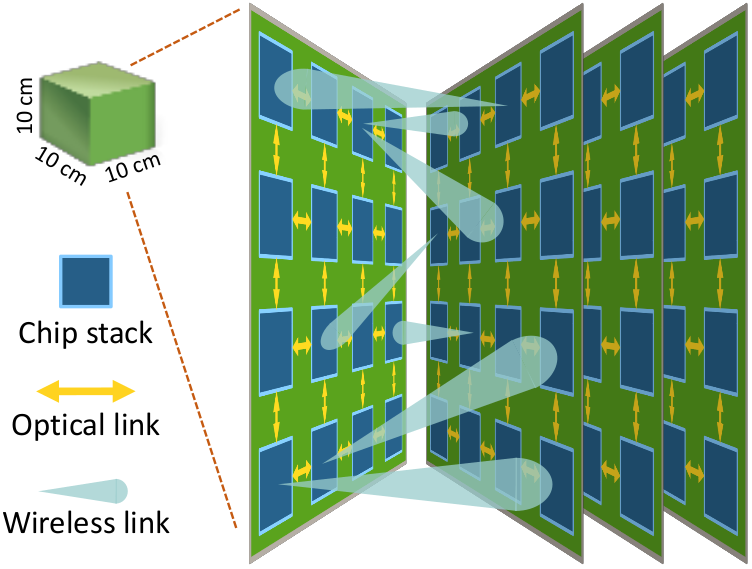
\includegraphics[width=0.4\textwidth]{haecbox}
    \caption[Processor architecture in the HAEC project]{Processor architecture employed in the \gls{haec} project. Numerous chip stacks are organized
    in compute boards and employ optical and wireless links for their interconnection. Each chip stack is a compute node consisting of of multiple
    cores arranged as a 3D mesh, which are interconnected by a wired \gls{noc}. The illustration is taken from the \gls{haec} presentation paper
    \cite[1]{matthiesen17haec}.}
    \label{fig:haecbox}
\end{figure}

The main contributions of this thesis are the conceptualization, implementation, and evaluation of a new approach for secure and efficient
communications in a \gls{noc} that is based upon the foundational work of \citeauthor{moriam18activeattackers}
\cites{moriam15manycorenc}{moriam18activeattackers}. This encompasses the design of an improved communication protocol in multiple variants and its
extensive evaluation through software simulation.

The thesis begins with an explanation of key terms and concepts that are essential for the comprehension of the remainder of this work (Chapter
\ref{ch:fundamentals}). Afterwards, a discourse on related research in the field of \glspl{noc} and their security is provided (Chapter
\ref{ch:relatedwork}). Subsequently, Chapter \ref{ch:overview} gives an overview of the methodologies and courses of action that were employed in this
thesis, followed by an exhaustive and detailed description of the designed communication protocol in Chapter \ref{ch:protocol}. Then, the
implementation of the simulator is presented (Chapter \ref{ch:implementation}) before evaluating the devised protocol (Chapter \ref{ch:evaluation}).
Finally, the thesis is concluded with a summary and an outlook on future work (Chapter \ref{ch:conclusion}).

    
    \chapter{Fundamentals}\label{ch:fundamentals}
    \section{Networks-On-Chip}\label{sec:networkonchipfun}
\textit{Network-on-Chip} (or \textit{\gls{noc}} for short) is a paradigm for interconnecting components on a chip. Typically employed on
\textit{Multi-Processor Systems-on-Chip (\glspl{mpsoc})} \cites(e.g.)(){ivanov05nocintroduction}{biswas15routerattack}{tatas16designingnocs}, they
provide the communication infrastructure for \textit{processing elements (\glspl{pe})} and possibly other \gls{ip} cores.

The topology of a \gls{noc} can vary. Researchers usually work with a 2D mesh topology
\cites(e.g.)(){frey17hardenednoc}{kumar02networkonchip}{fernandes16nocrouting}{boraten16packetsecurity}, which will also be used throughout this thesis.
In this case, each network node is connected to its four neighbors (excluding the boundary nodes).

A node typically consists of a processing element (often referred to as an \textit{\gls{ip} core} or just \textit{core}), a network interface,
and a router \cite{dally01routepacketsnotwires}. The router manages the connections to neighboring nodes while also allowing
the local processing element to communicate with the network through the network interface. An example of this architecture is given in Figure
\vref{fig:nocexample}.

Compared to traditional bus-based interconnect systems, \glspl{noc} can provide a lot of advantages, especially for many-core systems
\cite[5\psqq]{tatas16designingnocs}. One big advantage is scalability; because the cores do not share a global bus, \enquote{local performance is not
degraded} \cite[6]{tatas16designingnocs} as more components are added, and \enquote{aggregated bandwidth scales with the network size}
\cite[6]{tatas16designingnocs}.

In addition, the absence of global interconnection wires facilitates the use of different clock domains. This enables the implementation of the
\textit{globally asynchronous, locally synchronous (\gls{gals})} paradigm, which becomes increasingly important in chip design
\cites[3]{kumar02networkonchip}[2]{ivanov05nocintroduction}.

Furthermore, with the constantly increasing design complexity of modern chips \cite{mack11mooreslaw}, specialized on-chip
interconnections become infeasible to implement. Designing such a system \enquote{would take too much time and mapping of applications to dedicated
architectures would be impossible} \cite[1]{kumar02networkonchip}. In contrast, \glspl{noc} aims to be general purpose interconnect systems; they
\enquote{facilitate […] modularity by defining a standard interface} \cite[1]{dally01routepacketsnotwires}.

\begin{figure}
    \centering
    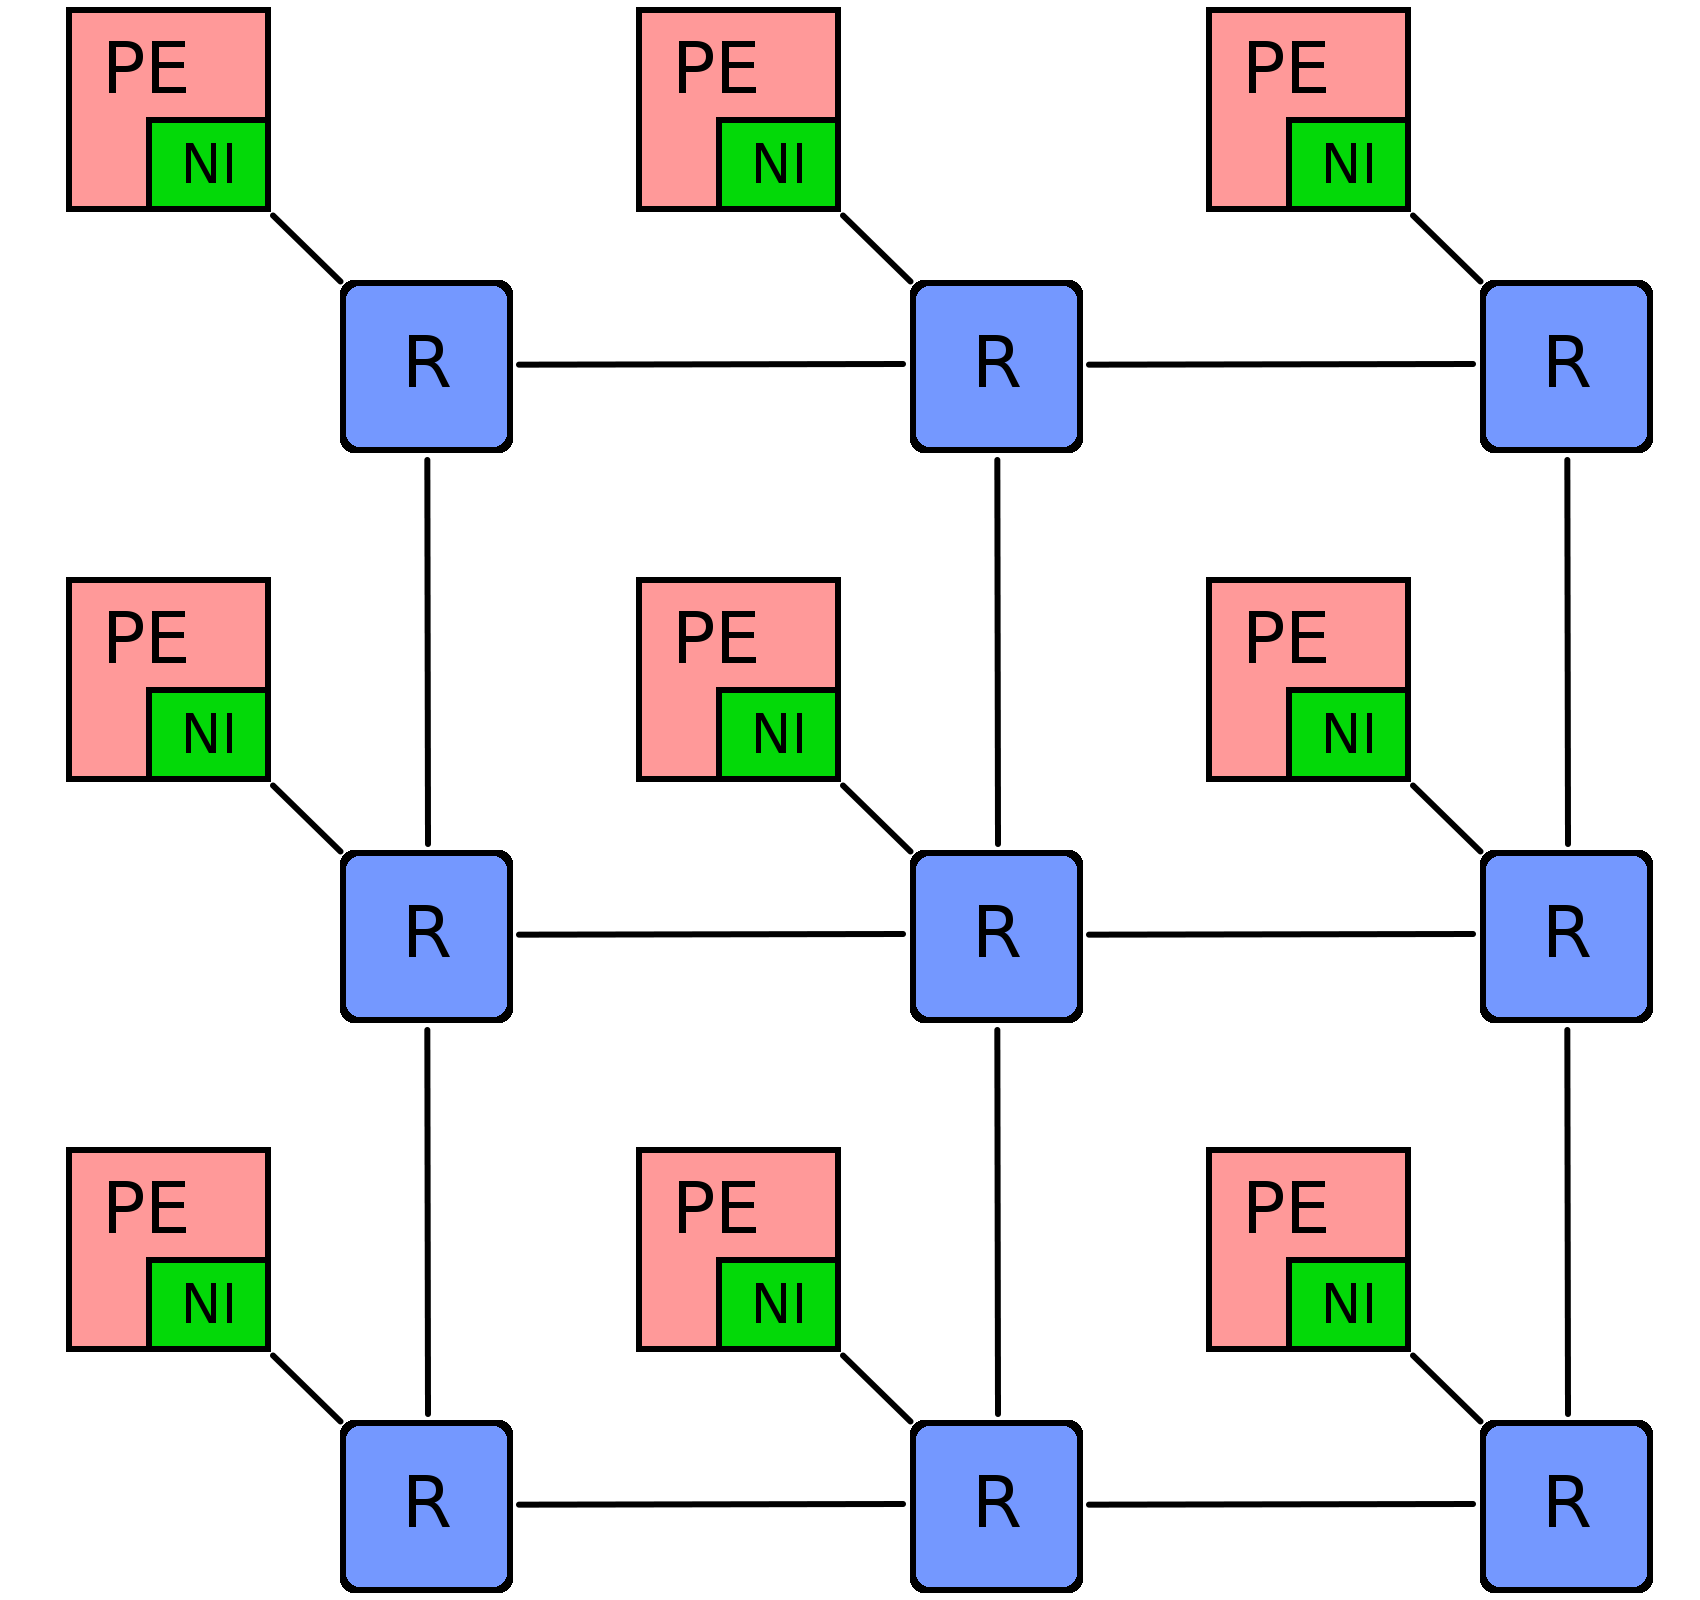
\includegraphics[width=0.6\textwidth]{noc_3x3_colored}
    \caption[Example of a 3x3 mesh NoC]{Example of a Network-on-Chip in a 2D mesh topology of size 3x3. The processing elements (red) contain a network interface
    (green) through which they are connected to a router (blue). The routers are interconnected as a 2D mesh.}
    \label{fig:nocexample}
\end{figure}

\section{Flits}\label{sec:flits}
Flits (short for \textit{flow control units}) are small pieces of data that are sent over a network. They are usually created by breaking a larger
packet down into parts that can be transmitted individually \cite[6]{flitslecturecmu}. Each flit must contain a set of header fields (such as source and
destination address, sequence number, or identifier) that are required for routing and handling \cite[2]{flitslectureutah}. In addition, it contains
a payload that carries the actual information to be transmitted.

In the context of \glspl{noc}, flits are often used as the standard unit of transmission \cite[51\psqq]{tatas16designingnocs}. Details on how flits
are used in this thesis can be found in (insert section/chapter vref).
% TODO: insert reference

\section{Hardware Trojans}\label{sec:hardwaretrojans}
% What are HTs, why can they get into other hardware, what are their properties
Hardware trojans are \enquote{malicious modifications of electronic hardware} \cite[1]{bhunia14hardwaretrojans} with the intent of disrupting normal
system behavior or extracting sensitive information. Because the integration of third party \gls{ip} has become increasingly popular due to circuit
complexity and cost efficiency \cites[1]{ancajas14fortnocs}[2]{bhunia14hardwaretrojans}, it is possible for adversaries to introduce hardware
trojans into larger systems, such as \glspl{mpsoc}.

In order to remain undetected, attackers aim to construct hardware trojans that are \enquote{stealthy in nature} \cite[1]{bhunia14hardwaretrojans}
and \enquote{evade […] detection through conventional postmanufacturing test} \cite[1]{bhunia14hardwaretrojans}. Hardware trojans are usually in a
dormant state until they are activated by a trigger signal to carry out their task \cites{bhunia14hardwaretrojans}{ancajas14fortnocs}. While the
trojan is inactive, communications through the \gls{noc} are unaffected and the system operates normally.

Attack types: information leak/eavesdropping, DoS (→ bandwidth depletion, deadlock, livelock)
% TODO: is this a fundamental? or write this when describing our attacker model?

\section{Network Coding}\label{sec:networkcodingfun}
Network coding is a technique for transmitting packets efficiently over a network. First described in 2000 by \citeauthor{ahlswede00networkflow}
\cite{ahlswede00networkflow}, the idea is to maximize the information flow through a network and achieve higher throughput than traditional transmission
schemes. It is achieved by allowing intermediate network nodes to encode incoming packets before passing them on, creating combinations of different
packets in the process. At the destinations, the received data can be decoded again to obtain the original packets.

A popular coding scheme, dubbed \textit{linear network coding} \cite{li03linearnc}, is to regard all packets arriving at a node from different incoming links as a vector.
Then, linear transformations can be applied to it to obtain new combinations to send out \cite[1]{li03linearnc}. To allow receivers to decode the
combinations into the original packets, the encoding patterns applied at each node can be \enquote{agreed upon beforehand} \cite[1]{li03linearnc}.
However, this requires global knowledge of the network topology. A practical alternative is to attach the encoding information to the packets in the
form of a \textit{global encoding vector (\gls{gev})} \cites[2\psqq]{chou03practicalnc}[5\psq]{chou07ncforinternetandwireless} that is updated at each intermediate node to
represent the current encoding pattern.

In addition to increasing the network performance by maximizing throughput, network coding can also provide an additional layer of resilience against
malicious intermediate nodes. It facilitates \enquote{a natural way to take advantage of multipath diversity for security against wiretapping attacks}
\cite[8]{fragouli07ncfundamentals} and can also be helpful against active attackers.

During this thesis, network coding is used primarily as a means of resilience against attackers. Furthermore, only the sender nodes will compute
combinations of different flits, while intermediate nodes merely forward them. Section (insert vref here) illuminates this subject in detail.
% TODO: insert vref


    \chapter{Related Work}\label{ch:relatedwork}
    \section{Network-on-Chip}\label{sec:networkonchiprel}
Research on new and efficient ways to interconnect components on a single chip has been an important field of research for decades. The concept of
general-purpose on-chip networks has been introduced in the early 2000s
\cites{dally01routepacketsnotwires}{kumar02networkonchip}{benini02nocparadigm} and has quickly gained a lot of traction in the research community
\cite[e.g.][]{ivanov05nocintroduction}. 
\Glspl{mpsoc} that utilize \glspl{noc} typically have a large number of processing elements that can run many different
tasks in parallel. \citeauthor{ancajas14fortnocs} have shown that the threat is relevant, especially in cloud computing setups, where several
untrusted applications may run at the same time. \cite{ancajas14fortnocs} % TODO: move this out of related work? also drop the untrusted applications part

In recent research, many different attack vectors have been explored, and a variety of countermeasures have been proposed to mitigate
attacks. The remainder of this section will explore them in detail.

% HT Survey & building trustworthy hardware
\citeauthor{bhunia14hardwaretrojans} \cite{bhunia14hardwaretrojans} have looked thoroughly into the threat of hardware trojans and possible protection
approaches. In a survey-like paper, they provide a detailed summary of attack scenarios, countermeasures, and detection paradigms. Similarly,
\citeauthor{sethumadhavan15trustworthyhardware} \cite{sethumadhavan15trustworthyhardware} analyze the challenge of building systems from untrusted
hardware conponents. They explain in detail how the hardware design and fabrication chain can be adapted to significantly lower the probability of
integrating malicious components. The methods in both works are not specific to \gls{noc} architectures, but are applicable to them nonetheless.

% Security framework (2003)
The necessity of security measures as part of the design was already recognized early on in \gls{noc} research. In 2003,
\citeauthor{gebotys03securityframework} \cite{gebotys03securityframework} proposed a \enquote{general security architecture}
\cite[1]{gebotys03securityframework} to impede attacks \enquote{at both the network level […] and at the core level}
\cite[1]{gebotys03securityframework}.

At the network level, they differentiate between secure cores and other cores. The secure cores are capable of encrypting and authenticating network
traffic, and are thus designed to handle sensitive user information. In addition, there is a dedicated key-keeper core that handles key distribution
amongst the secure cores. At the core level (or application level), the authors propose to use a modified implementation of elliptic curve
cryptography to facilitate encryption and authentication. Aiming to provide resistance against side channel power attacks, their modifications conceal
the power traces of the different algebraic computations during the cryptographic operations. This hinders adversaries from extracting key bits based
on power spikes.

\citeauthor{kapoor13nocauthenc} \cite{kapoor13nocauthenc} have persued a similar approach. They also separate the cores into secure and non-secure
ones (often referred to as \textit{security zones}) and propose to implement authenticated encryption in the network interfaces. While the secure
cores employ permanent keys to communicate with each other, the non-secure ones may use plain text messages. Additionally, in order to allow
communication between the security zones, sessions may be established with individually generated session keys. Furthermore, the authors employ
traffic limitations in the network interfaces to prevent \gls{dos} attacks by malicious cores, while access rights tables prohibit unauthorized
memory accesses.

Another popular approach is to divide the \gls{noc} into security zones. Not to defend against HTs, but potentially malicious applications running on
parts of the NoC. Apps working with critical information → secure zone.

% Fort-NoCs
\citeauthor{ancajas14fortnocs} \cite{ancajas14fortnocs} have investigated the threat of hardware trojans for \glspl{noc}. They show that the usage of
third party \gls{noc} \gls{ip} is very popular due to cost efficiency, opening up an infection vector for hardware
trojans. Together with a software accomplice (i.e. an infected processing element) that can send commands to the trojan, this may
lead to information leaks, data corruption or denial of service attacks.

The authors focus on mitigating \enquote{covert data theft by a compromised \gls{noc}} \cite[3]{ancajas14fortnocs}. They suggest a three-layer
approach to mitigate this threat, consisting of data scrambling, packet certification, and node obfuscation. These techniques are
implemented solely in the network interfaces, which are not provided by a third party and hence assumed to be trustworthy. The goal of these measures
is to prevent activation of the hardware trojan and render transmitted information unreadable to the attacker.

% Hardened NoC design
\citeauthor{frey17hardenednoc} \cite{frey17hardenednoc} also worked on mitigating the effect of hardware trojans in a \gls{noc}. Their goal is to
harden the \gls{noc} design against potential hardware trojans located inside the routers. In contrast to \citeauthor{ancajas14fortnocs}
\cite{ancajas14fortnocs}, the protective measures are implemented at the router level and not in the network interfaces. They are designed to
\enquote{complement […] the previous \gls{noc} works aiming for \gls{ni} security} \cite[16]{frey17hardenednoc} and address \gls{dos} attacks rather
than information leakage.

The idea of the authors is to detect any flit tampering right after the flit leaves a router. To achieve this, an error control code and dynamic flit
permutation are applied to all flits before they enter a router, and the reverse transformations are applied after they exit the router again. This
prevents (or at least detects) small and targeted modifications to the flit headers. % TODO: not the best wording

% Runtime hardening
Another \gls{noc} hardening approach was investigated by 

While \citeauthor{ancajas14fortnocs} have devised a method to preemptively protect an \gls{mpsoc} against potential hardware trojans, XY focus on
detecting them.

\section{Network Coding}\label{sec:networkcodingrel}
% TODO: put this completely in fundamentals?

\section{Lightweight Cryptographic Algorithms}\label{sec:lightweightcrypto}
For security reasons, it is often desirable to add encryption and authentication to the communication passing through a \gls{noc}. However,
standard cryptographic algorithms such as \gls{aes} are usually not efficient enough for this task. \cite[1]{bogdanov07present}
In the work preceding this thesis, lightweight cryptographic algorithms were thoroughly explored. \cite{harttung17lightweightcrypto} Such
algorithms are
specifically designed to have efficient hardware implementations with low area and power requirements. In addition, they aim to have a small
computation delay while still providing an adequate level of security. Examples of such algorithms are PRESENT \cite{bogdanov07present},
mCrypton \cite{lim06mcrypton}, PRINCE \cite{borghoff12prince} and Klein \cite{gong12klein}. Some of them will be explained further later in this
thesis. % TODO: reference this when explaining PRINCE later on

\section{Notes}
\begin{itemize}
    \item \textbf{\citetitle{ivanov05nocintroduction}}
        \begin{itemize}
            \item Aus dem Jahr 2005, als SoC-Kommunikationsschwierigkeiten wichtiger wurden
            \item Wird als langfristiger Einstiegspunkt in NoC-Forschung gesehen von den Autoren
        \end{itemize}
    \item \textbf{\citetitle{sethumadhavan15trustworthyhardware}}
        \begin{itemize}
            \item Introduction into hardware design process and compromisation vectors
            \item Explains how the hardware design and fabrication chain is vulnerable to exploits/attacks
            \item Three security systems operating "in series" (next one is only coming into play if previous one has failed)
                \begin{enumerate}
                    \item Static check that the design being used is backdoor-free
                    \item Runtime altering of inputs (→ obfuscation) to ensure backdoors are not triggered/turned on
                    \item Runtime on-chip monitoring (of instruction counts, opcode types, ...) to detect enabled backdoors
                \end{enumerate}
        \end{itemize}
    \item \textbf{\citetitle{ancajas14fortnocs}}
        \begin{itemize}
            \item MPSoCs with 3rd party IP NoCs (i.e. the interconnect system is 3rd party)
            \item Software accomplices (malicious/infected processing elements)
            \item Attack types: eavesdropping (information leak), voluntary data corruption, denial of service
            \item Fort-NoCs: 3-layer security mechanism (hardware level protection)
                \begin{itemize}
                    \item Lower layer data scrambling (hardware encryption to prevent covert activation sequences from AcTh to Trojan)
                    \item Middle layer packet certification (authentication tag, detect unintended destination after flit copy)
                    \item Top layer node obfuscation (migrate running applications from one node to another)
                \end{itemize}
            \item Malicious PE must secretly communicate with hardware trojan to send commands (C\&C node)
            \item Easy to run malicious software on a PE e.g. in cloud computing setups
            \item Small area and power overhead, mostly small runtime overhead
            \item Not all layers need to be used (in lower security domains)
        \end{itemize}
    \item \textbf{\citetitle{frey15stateobfuscation}}
        \begin{itemize}
            \item Attacker model: HT is the FSM control unit of NIs (very specific HT location)
            \item Countermeasure: obfuscate the states and state transistions that the FSMs do
            \item HT modifying state transitions causes FSM to enter illegal/invalid state → HT warning
            \item High HT detection rate (for this specific type of HT)
        \end{itemize}
    \item \textbf{\citetitle{frey17hardenednoc}}
        \begin{itemize}
            \item Published two years after state obfuscation paper above
            \item Router level hardware trojans (HTs)
            \item Focuses on DoS attacks (bandwidth depletion) originating in a router (not a NI because router has more connections → more
                feasible)
            \item Implement DoS mitigation directly in the routers, rather than NI, to prevent bandwidth depletion as quickly as possible
            \item Physically Unclonable Function (PUF): random vector generation in each router
            \item Apply random dynamic permutation (data scrambling) to flits arriving at a router input (makes modifying flits into something
                meaningful significantly harder) before flit reaches the input queue (where the HT has access); de-permutate at output port (→
                PUF random vectors)
            \item Apply ECC (error control code) encoding before input port; decode before output port (only critical flit bits: header, tail,
                dest. address)
            \item Check flit integrity after leaving input queue and right before departing through the computed output port
            \item Cites lots of useful other related work
        \end{itemize}
    \item \textbf{\citetitle{fernandes16nocrouting}}
        \begin{itemize}
            \item "Attacks at MPSoC aim to extract sensitive data, modify the system behavior or denial the system operation (Denial-of-Service,
                DoS)"
            \item Build security zones in the NoC using routing algorithm ("wrap IPs and protect sensitive information from attacker")
            \item Firewalls also possible, but may be costly (→ they implement a security policy in the NI)
            \item Aims to protect against software-based attacks (NoC is assumed to be secure)
            \item Threat model: timing and DoS attacks
            \item Security zone is e.g. the set of IP blocks that an application was mapped on
            \item Routing algorithm tries to keep the sensitive path completely inside the same security zone, if possible
        \end{itemize}
    \item \textbf{\citetitle{boraten16packetsecurity}}
        \begin{itemize}
            \item Packet-Security (P-Sec)
            \item Threat model: compromised NoC does fault injection (side channel attack)
            \item It is possible to eventually obtain encryption keys by observing how encoders and decoders react to the side channel attacks
            \item → ensure integrity of packets using error correction codes (ECCs) (→ AMD, CRC)
            \item AMD for sensitive communications (together with encryption), otherwise CRC to provide minimal fault tolerance
        \end{itemize}
    \item \textbf{\citetitle{boraten18mitigationdos}}
        \begin{itemize}
            \item Published 2 year after Packet Security paper above (builds upon previous research)
            \item HT does DoS attack: inspect packets, inject fault, trigger ECC response (ECC cannot correct error) → repeated transmissions,
                deadlocks
            \item HT resides in links between nodes
            \item Prevention: Heuristic fault classification → discover HTs
            \item Continue using compromised links instead of rerouting → obfuscation to prevent HT triggering, optimized AMDs to detect fault
                injections
            \item Little overhead: 2\% area, 6\% power
            \item "[...] we can classify security threats for NoCs as a subset of preexisting challenges originating from but not limited to,
                on-chip fault tolerance, functional correctness, path diversity, isolation, and quality of service"
            \item Security measures should not be compromised themselves
        \end{itemize}
    \item \textbf{\citetitle{biswas15routerattack}}
        \begin{itemize}
            \item Survey of MPSoC attack types
            \item New attack type for routing table-based routers (i.e. reconfigurable routers as opposed to routers with fixed routing logic)
            \item Mentions survey of hardware trojan detection techniques
            \item Not about detecting HTs, but about protection from malicious users
            \item → TEEs and REEs (Trusted/Rich Execution Environments), similar to security zones
            \item It is desirable to use routing tables instead of fixed routing logic (flexibility, more complex routing algorithms)
            \item Attack scenario: routing table is loaded onto NoC at boot or runtime (by host processor or NoC controller), which is modified by
                the attacker → unauthorized access and misrouting (routing to other environment)
        \end{itemize}
    \item \textbf{\citetitle{gebotys03securityframework}}
        \begin{itemize}
            \item Framework: protection both at network and application layer
            \item Network layer
                \begin{itemize}
                    \item Key-keeper core: protects/distributes encryption keys to other secure cores
                    \item Each secure core has a security wrapper
                    \item Focus on key distribution and key management
                \end{itemize}
            \item Application layer
                \begin{itemize}
                    \item Software modifications for resistance against power (side-channel) attacks
                \end{itemize}
            \item Higher level approach than most other papers (more protocol layer than hardware layer)
            \item Strong assumptions on trusted software and hardware
            \item No clear attacker model, paper seems more like a "framework suggestion"
        \end{itemize}
    \item \textbf{\citetitle{kapoor13nocauthenc}}
        \begin{itemize}
            \item 2 NoC zones: secure and non-secure IP cores
            \item Authenticated Encryption implemented in NIs of secure cores
            \item Secure cores can communicate with each other using permanent keys
            \item Non-secure cores can communicate with each other using plain text
            \item Hardware (NIs + routers) are assumed to be secure
            \item Secure and non-secure cores communicate with session keys and an intermediate link IP core (link can be secure or non-secure)
            \item Memory IP cores have access rights table in NI to prevent unauthorized memory accesses
            \item DoS attacks prevented by having a max number of packets allowed to be sent implemented in NI
        \end{itemize}
    \item \textbf{\citetitle{evain05nocsecurityanalysis}}
        \begin{itemize}
            \item In their context: CCM (central configuration module) is added (unique IP block → initialize and (re)configure NoC). Also CCM:
                add supervising and defending reactions for security
            \item FPGA vs. ASIC: reconfigurability of FPGA is another potential attack vector
            \item Mixed FPGA/ASIC implementation possible: ASIC for secure zone, FPGA for insecure zone (CCM must be in secure zone)
            \item Many possible attack types → different protection strategies
                \begin{itemize}
                    \item Bandwidth denial: virtual channels in the secure area (unsecure packets can't obstruct secure packets)
                    \item Unauthorized access: packet/path filters at zone boundaries and/or at NIs
                    \item Only encrypted/authenticated communication with the CCM
                \end{itemize}
        \end{itemize}
    \item \textbf{\citetitle{stefan11enhancingnocs}}
        \begin{itemize}
            \item Introduce non-determinism through multipath routing
            \item Proposal is implemented on top of Aethereal framework
            \item Time-division multiplexing (TDM) for router channels
            \item Alternative path selection
                \begin{itemize}
                    \item … based on position in the slot table at the moment of sending (static schedule)
                    \item … based on hardware RNG (dynamic at runtime)
                \end{itemize}
        \end{itemize}
\end{itemize}

Different attacker/threat models in literature. Depending on the attacker model, different approaches are used to protect the system against it.
E.g. when the underlying network architecture (the NoC itself) is assumed to be compromised, protection is implemented in the network interfaces
of the nodes. If the attacker only has access to specific parts of the routers or specific zones of the NoC, protection can be implemented through
the routing algorithm. → The power of the HTs differs. The more complex the HT is, the stronger it influences chip area/power consumption/runtime
overhead and may be easier detectable → that's why HTs are often assumed to use "small" attacks like fault injection, or have access to only very
specific components of the NoC to stay undetected/not require much chip area.

Differentiate between methods to detect HTs (on software level, firmware level, w/ static analysis, side-channel analysis), and methods to harden
the NoC against potential HT infections.

NI is usually assumed to be trusted, and routers are potentially compromised because of 3rd party IP or 3rd party manufacturing/integration
partners. Other threat model: software attacks (NoC itself is secure).

How to get HT into hardware: rogue employee, 3rd party IP, 3rd party manufacturing/integration partners, ...

This thesis: no hardware synthesis, use software simulation. Focus on malicious flit modification (→ attacker model) rather than DoS attacks. Our
model assumes that the NoC routers and links may be compromised and thus relies on the NIs for the security measures → no effective protection
against bandwidth depletion, but this is not the goal.
Deterministic vs. static routing? No security zones or division into secure/non-secure zones/cores.

The concept of security zones can be implemented in different ways. Bla et al. propose to do X, while bla enforce them through the routing protocol.



    \chapter{The HAEC Project}

    \chapter{Simulation Setup}
    \section{Node Layout}

    \section{Attacker Model}
    \begin{itemize}
        \item Variable number of compromised routers (e.g. 8 for an 8x8 grid)
        \item Compromised routers randomly drop or modify packets (no intelligent modifications/drops)
    \end{itemize}

    \chapter{NoC Design}
    2D mesh as NoC topology is very common in research (insert many cites here).
    \begin{itemize}
        \item Encryption/authentication ordering
            \begin{itemize}
                \item Encrypt-then-MAC: best practice. Sequential encrypt/authenticate on sender side, but parallel decrypt/verify
                    on receiver side. Advantage: MAC can be computed on sender side immediately when ciphertext arrives, even when
                    MAC flit has not arrived yet (if ARQ is necessary, it can be issued right away)
                \item MAC-then-encrypt: bad. Sequential authenticate/encrypt on sender side and sequential decrypt/verify on receiver
                    side.
                \item Encrypt-and-MAC: okay. Parallel encrypt/authenticate on sender side, but sequential decrypt/verify on receiver
                    side (overall same latency as Encrypt-then-MAC, but without advantage of fast ARQs)
            \end{itemize}
        \item GALS (Globally Asynchronous, Locally Synchronous)
            \begin{itemize}
                \item not relevant for simulations, just for actual hardware (e.g. power spikes on active clock edges, low-power PEs etc.)
                \item simulation is only inaccurate at the link between routers
                \item we just do Globally Synchronous because it's easier
            \end{itemize}
        \item 24 bit FIDs/GIDs
            \begin{itemize}
                \item integer overflow after $2^{24}-1$
                \item this is the latest time when session keys should be changed, otherwise packet injection (repeat attacks) become
                    possible
            \end{itemize}
        \item Retransmission Buffer structure and lookup times
            \begin{itemize}
                \item corresponding flits are stored consecutively (e.g. data/MAC of same FID, flits of same generation etc.)
                \item lookup time (in clock cycles) is a parameter in the simulation
                \item UC case: one cycle lookup is fine (just need to find FID, mode field determines offset in the buffer)
                \item NC case: two cycles for lookup (one to find GID, one to compare GEVs of the generation in parallel, mode determines offset)
            \end{itemize}
        \item Priorities
            \begin{itemize}
                \item retransmission buffer: ARQs have priority
                \item crypto units (→ entry guard): arriving flits have priority
            \end{itemize}
        \item Lane widths
            \begin{itemize}
                \item lanes have as many wires as flits have bits
                \item one flit can be transmitted per clock cycle per lane
                \item flit size is fixed (standard header fields + 64 bit payload)
            \end{itemize}
        \item Buffers/Queues
            \begin{itemize}
                \item App/NI/Routers have only input buffers, no output buffers
                \item Routers only route flits when the receiving router's input queue is not full
            \end{itemize}
        \item Crypto units
            \begin{itemize}
                \item Separate units for encryption and decryption
                \item Send/receive pipeline share the same set of crypto units
            \end{itemize}
        \item Routing Strategies
            \begin{itemize}
                \item XY/YX
                    \begin{itemize}
                        \item Deterministic path
                        \item Attacker controlling a single router can reliably disrupt communication between certain nodes
                        \item does not distribute flits of a generation across different paths
                    \end{itemize}
                \item XY/YX + Valiant
                    \begin{itemize}
                        \item Deterministic path only if fixed valiant
                    \end{itemize}
                \item Random XorY
                \item Random XorY + Valiant
            \end{itemize}
        \item Injection rate
            \begin{itemize}
                \item Value if 0.2 is realistic
                \item Possibility to generate pairs for fair comparison of UC/NC
            \end{itemize}
    \end{itemize}

    \chapter{Communication Protocol}
    \begin{itemize}
        \item Uncoded transmission
            \begin{itemize}
                \item no network coding
                \item 2 methods: 1 data flit + 1 MAC flit OR 2 data/MAC split flits
            \end{itemize}
        \item Flit structure
            \begin{itemize}
                \item burst bit, source/target address, mode, address, GID/FID, GEV, payload
                \item mode: define if data/mac/split/arq
            \end{itemize}
        \item Network coded transmission
            \begin{itemize}
                \item Number of flits: G2C3 or G2C4
                \item 3 methods: 1 data flit + 1 MAC flit OR 1 MAC flit per generation OR 2 data/MAC split flits
            \end{itemize}
        \item ARQs
            \begin{itemize}
                \item Limited number of ARQs per transmission unit (UC: data/MAC pair or split pair, NC: generation)
                \item Timeout of x (e.g. 8) cycles until first ARQ is sent
                \item If limit >1: start larger timeout (→ round-trip of ARQ)
                \item Many different cases, insert some flow diagrams here
                \item The higher the ARQ timeout/limit, the less likely the flit is still in retransmission buffer
                \item → ARQ timeout/limit and retransmission buffer size have to correlate
                \item In the case that we only have 1 ARQ left that we are allowed to send: Wait for any ongoing MAC verifications
                    so in case they fail, the flits can be included in the ARQ
            \end{itemize}
    \end{itemize}

    \chapter{Statistics}
    \begin{itemize}
        \item Injection/acceptance rate: [0, 1] (at processing element and at network interface)
        \item Queue lengths and buffer sizes
        \item Workload of crypto units
        \item Average/max flit waiting time at entry guard
        \item Average/max hop count
    \end{itemize}

    \chapter{Implementation}
    \section{Course of Events}
    \begin{itemize}
        \item lalala
    \end{itemize}

    \section{Components}
    \subsection{Network Interface}

    \chapter{Future Work}
    \begin{itemize}
        \item Local network coding, local encoding vectors
        \item Burst mode
    \end{itemize}

    \chapter{Talk About}
    \begin{itemize}
        \item Encrypt-then-MAC vs. Encrypt-and-MAC (bei Encrypt-then-MAC encrypt+authenticate sequentiell, aber decrypt+verify parallel.
            Bei Encrypt-and-MAC encrypt+authenticate parallel, aber decrypt+verify sequentiell). Bei Encrypt-and-MAC: decrypt kann schon
            beginnen, wenn MAC noch nicht da ist, verringert die Latenz in manchen Fällen.
        \item Overhead von Verschlüsselung+Auth vs. nur Auth vs keins von beiden (sowohl Latenz als auch Chipfläche)
        \item Welche Komponenten brauchen wie viele Takte
        \item Anzahl der Enc/Auth units bei den verschiedenen Methoden (mehr enc als auth bei Methode 2)
        \item GALS design pattern - wir sind aber auf jeden Fall synchron innerhalb einer Node, d.h. wenn GALS vs GS diskutiert wird,
            ändert sich nur die Zeit der Übertragung zwischen den Routern → zur Vereinfachung wird GS angenommen
        \item Leichtgewichtige Krypto: FPGA vs. ASIC, speedup von Faktor 3-4 wahrscheinlich möglich (→ critical path delay) \cite{kuon07fpgavsasic}
            → AES und AES\_INV zum Vergleich, da ähnlicher Aufbau von kombinatorischer Logik + FlipFlops (Rundenfunktionen etc.)
        \item Statistiken: Wie viele Crypto Units für Auth+Enc sind gleichzeitig besetzt (→ Auslastung)
        \item Threat model, protection goals
        \item node-unique FIDs/GIDs have advantage that 24 bits are not full nearly as fast as with globally unique IDs
		\item large flits (128 bits) need 2 crypto units (w/ block size 64 bit)
        \item Lack of error correcting code (ECC) in simulation
        \item Deadlock/Livelock possibilities? D yes, L not
    \end{itemize}

    \section{Assumptions}
    \begin{itemize}
        \item only input buffers are used (for app, NI, router), no output buffers
        \item network coding module stores flits until enough flits with the same
            destination are available (in our case: 2)
        \item network coding (creating all 3 combinations) takes one cycle, but
            because we can only send one flit out per cycle, it takes 3 cycles until
            all combinations are sent (so in the end it's one combination per cycle)
        \item we have a variable number of authentication units and the amount of
            cycles the encryption algorithm takes can be set by a parameter
        \item if all crypto units are busy, the encoded flit combinations are held
            back in a dedicated buffer
        \item if e.g. authentication method 1 is used (1 MAC flit per data flit),
            the data flit is sent out one cycle before the MAC finished computing,
            so the MAC can be sent immediately when it's ready
        \item the encoding/authentication and decoding/verification pipelines in the
            network interface share the same crypto units (but this is not
            implemented yet)
        \item when a flit arrives at the NI from the router, the first thing that is
            done is checking if this is an ARQ. If yes, it is delivered directly to
            the retransmission buffer. Otherwise, it goes through the normal network
            decoding pipeline
        \item when an ARQ arrives at a NI, it takes one cycle to look up the correct
            flit and it will be sent out in the same cycle (not sure about this, two
            cycles might be more realistic)
        \item size of the retransmission buffer is configurable
        \item retransmission buffers use a FIFO caching strategy
        \item if an ARQ and a new data flit arrive a the retransmission buffer
            during the same clock cycle, the ARQ answer (retransmission) has
            priority to be sent out first
        \item in a router, several flits can be routed simultaneously, provided that
            they do not share an input or output port
        \item also in router: flits are held back in the input queues if the
            receiving router's input queue is full (this was discussed in an earlier
            email)
        \item in uncoded flits, the GID header contains a flit ID instead of
            generation ID, and MAC and data flit have the same ID
        \item the different values for the mode header are: normal data flit, mac
            flit, data/mac combined, ARQ
        \item entry guard can distribute a departing and an arriving flit at the same
            time, as long as units are free
        \item it does not matter whether data or mac flit is sent out first (order),
            because they can arrive out-of-order at the destination node anyway
        \item encryption units can also be used for decryption
    \end{itemize}

    \chapter{Notes}
    \section{NoC Design}
    \begin{itemize}
        \item Router: in+out buffer vs. only input buffer (2 cycles vs. 1 cycle routing)
        \item GenTraffic: injection rate of 0.2 was considered in Sadia's calculations and is a good starting point
        \item Network Interface: sender and receiver share the crypto units → we need to keep track of where the flit has to go after leaving the crypto unit → flag at crypto unit itself?
        \item Speed: \gls{noc} usually runs at ~500 MHz or a bit lower, but definitely runs a lot faster than the maximum frequency of the lightweight encryption algorithms. Using multiple clock domains is hard and requires expertise
        \item Crypto algorithms: 18 units for mCrypton was planned; also possible to use multiple (but less) PRINCE units, but then the clock domain problem arises again
    \end{itemize}

    % % % Glossary % % %
    %\glsaddall % Print all glossary entries, not only the referenced ones
    \printglossaries
	
	% % % Bibliography % % %
	%\nocite{*} % Put all entries in the bibliography, not only those cited in the document
    \printbibliography[heading=bibintoc]
\end{document}
